\documentclass[12pt,a4paper]{article}
\usepackage[french]{babel}
\usepackage[utf8]{inputenc}
\usepackage[T1]{fontenc}
\usepackage{graphicx}

\title{Spécifications du Projet Planning Nouvelle Génération (PNG)}
\author{Tom BARTIER, ROBIN Yann, Marçais André, BA GUBAIR Emad}
\date{\today}

\begin{document}

\maketitle

\begin{abstract}
    Ce document décrit les spécifications des usecases "Consulter l'emploi du temps par salles" et 
    "Insérer un cours".
\end{abstract}

\section{Maquette}
Voici la maquette initialement pensée de consulter 

\section{UC "Consulter l'emploi du temps par salles"}
Description : L'utilisateur connecté consulte l'emploi du temps de la salle voulue sur la semaine voulue.\\
Acteur : Utilisateur \\
Déclencheur : L'utilisateur clique sur "Salle"\\
Pré-Condition : L'utilisateur est connecté\\
Post-Condition : L'emploi du temps de la salle et de la semaine choisie est affiché
\\

Scénario nominal\\
1. L'utilisateur clique sur le bouton "Salles"\\
2. Le système affiche la liste des salles\\
3. L'utilisateur clique sur le nom de la salle qui l'intéresse\\
4. Le système affiche l'emploi du temps de la salle sur une semaine\\

Scénarios alternatifs\\
Changer salle affichée\\
3. L'utilisateur clique sur le nom de la salle\\
4. Le système affiche toutes les salles\\
5. L'utilisateur clique sur le nom de la salle qui l'intéresse\\
6. Le système affiche l'EDT de la salle sur la semaine\\

Choix semaine\\
3. L'utilisateur clique sur le numéro de la semaine qui l'intéresse\\
4. Le système affiche l'EDT de la salle sur la semaine choisie\\


\begin{figure}[h]
    \centering
    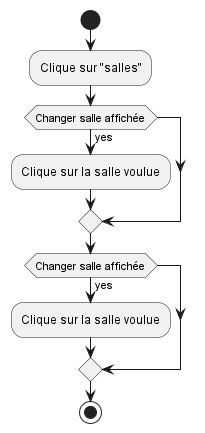
\includegraphics[width=0.3\textwidth]{Diag_activites_UC03.png}
    \caption{Diagramme d'activités UC03}
    \label{fig:act_03}
\end{figure}

\section{UC11 "Ajouter un cours"}
Description : le responsable ajoute un créneau cours dans l'emploi du temps\\
Acteur : Responsable d'EDT\\
Déclencheur : Le responsable clique sur un créneau vide ou sur le bouton "Ajouter nouveau cours"\\
Pré-Condition : Le responsable est connecté et un créneau vide est disponible\\
Post-Condition : Le créneau de cours a été crée dans l'emploi du temps\\

Scénario nominal : \\
1. Le responsable clique sur le bouton "Ajouter un cours"\\
2. Le système affiche une fenêtre pour rentrer les informations du cours\\
3. Le responsable clique sur le bouton "Module"\\
4. Le système affiche la liste des modules\\
5. Le responsable clique sur le module du cours\\
6. Le responsable clique sur le bouton "Professeur"\\
7. Le système affiche la liste des professeurs\\
8. Le responsable clique sur le professeur du cours\\
9. Le responsable clique sur le bouton "Horaire"\\
10. Le système affiche la liste des jours et heures\\
11. Le responsable clique sur le jour et l'heure de début et de fin du cours\\
12. Le responsable clique sur le bouton "Salle"\\
13. Le système affiche la liste des salles disponibles\\
14. Le responsable clique sur la salle du cours\\
15. Le responsable clique sur le bouton "Valider"\\
16. Le système affiche le cours ajouté\\

Scénario alternatif\\
15. Le responsable clique sur le bouton "Propager"\\
16. Le système affiche deux menus déroulants de semaine\\
17. Le responsable sélectionne la semaine de début et la semaine de fin\\
18. Le responsable clique sur le bouton "Valider"\\
19. Le système affiche les cours ajoutés\\

Scénario d'exception\\
15. Le responsable clique sur le bouton "Annuler"\\
16. Le système ferme la fenêtre\\

\begin{figure}[h]
    \centering
    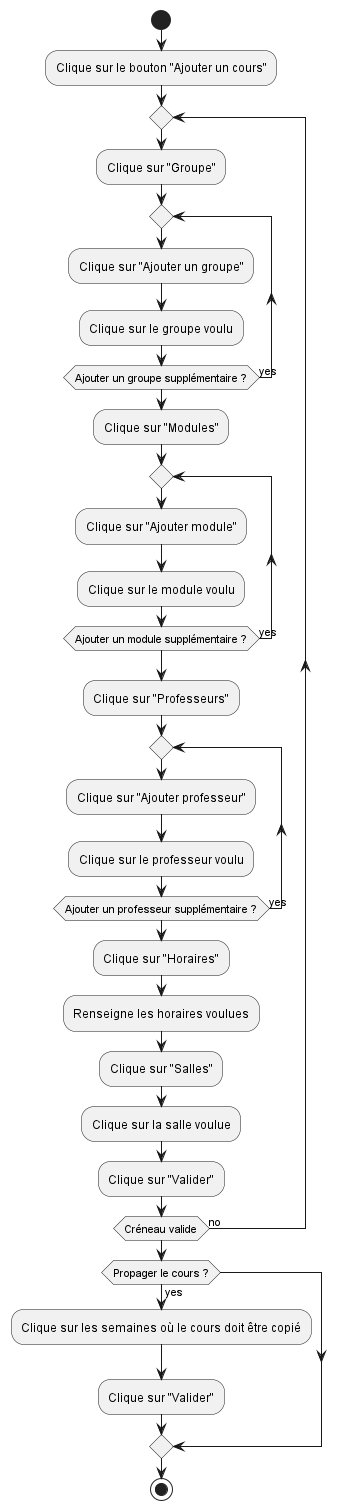
\includegraphics[width=0.4\textwidth]{Diag_activites_UC11.png}
    \caption{Diagramme d'activités UC11}
    \label{fig:act_011}
\end{figure}

\end{document}